\newcommand{\datasetSplitDiagram}{%
  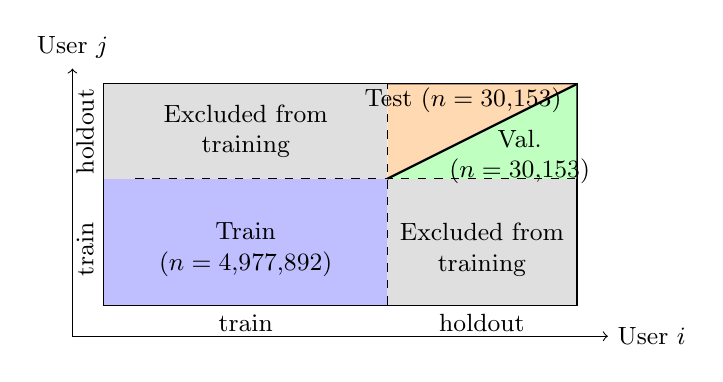
\begin{tikzpicture}[x=0.8cm,y=0.4cm,font=\small]
    \draw[->] (0,0) -- (8.5,0) node[right] {User $i$};
    \draw[->] (0,0) -- (0,8.5) node[above] {User $j$};

    \draw[thick] (0.5,1.0) rectangle (8,8);

    \fill[blue!25] (0.5,1.0) rectangle (5,5);

    \fill[gray!25] (0.5,5) rectangle (5,8);
    \fill[gray!25] (5,1.0) rectangle (8,5);

    \fill[green!25] (5,5) -- (8,5) -- (8,8) -- cycle;
    \fill[orange!30] (5,5) -- (5,8) -- (8,8) -- cycle;

    \draw[dashed] (5,1.0) -- (5,8);
    \draw[dashed] (1.0,5) -- (8,5);
    \draw[thick] (5,5) -- (8,8);

    \node[align=center] at (2.75,2.75) {Train\\$(n=4{,}977{,}892)$};
    \node[align=center] at (2.75,6.5) {Excluded from\\training};
    \node[align=center] at (6.5,2.75) {Excluded from\\training};
    \node[align=center] at (7.1,5.7) {         Val. \\$(n=30{,}153)$};
    \node[align=center] at (6.2,7.5) {Test $(n=30{,}153)$};

    \node[below] at (2.75,1) {train};
    \node[below] at (6.5,1) {holdout};
    \node[rotate=90] at (0.2,2.75) {train};
    \node[rotate=90] at (0.2,6.5) {holdout};
  \end{tikzpicture}%
}
